\documentclass{standalone}
\usepackage{tikz}
\usetikzlibrary{patterns, positioning}
\usepackage[sfdefault]{ClearSans} %% option 'sfdefault' activates Clear Sans as the default text font
\usepackage[T1]{fontenc}

\begin{document}
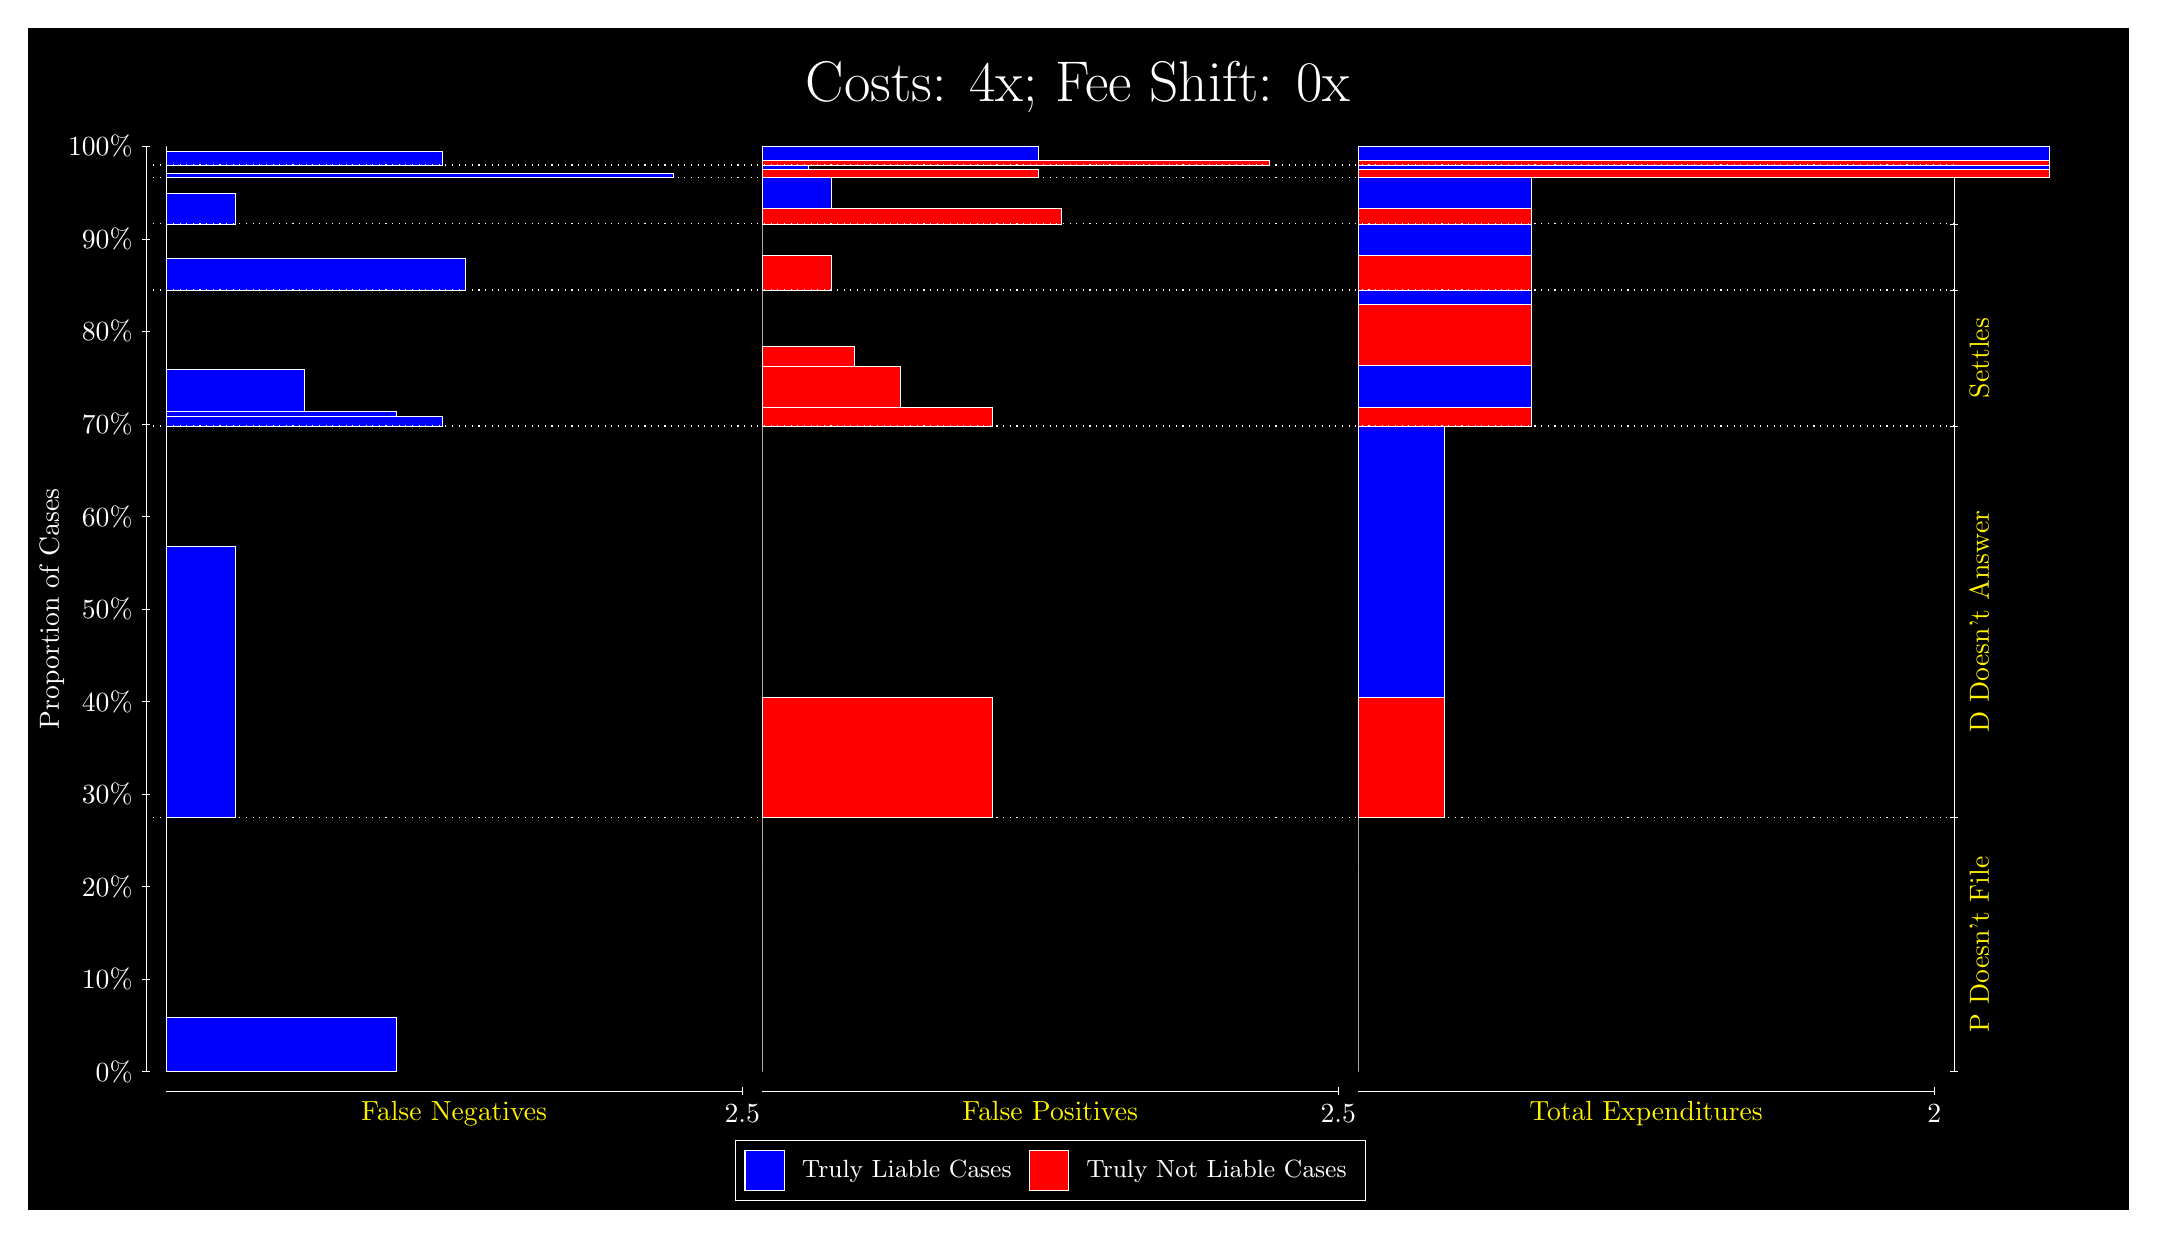
\begin{tikzpicture}
\draw[fill=black] (0,0) rectangle (26.667,15);
\draw[text=white] (0,13.5) rectangle (26.667,15) node[midway] {\huge Costs: 4x; Fee Shift: 0x};
\draw[white, very thin] (1.5,1.75) -- (1.5,13.5);
\node[rotate=90, text=white, anchor=center] at (0.3, 7.625) {Proportion of Cases};
\draw[white, very thin] (1.45,1.75) -- (1.55,1.75);
\node[text=white, anchor=east] at (1.45, 1.75) {0\%};
\draw[white, very thin] (1.45,2.925) -- (1.55,2.925);
\node[text=white, anchor=east] at (1.45, 2.925) {10\%};
\draw[white, very thin] (1.45,4.1) -- (1.55,4.1);
\node[text=white, anchor=east] at (1.45, 4.1) {20\%};
\draw[white, very thin] (1.45,5.275) -- (1.55,5.275);
\node[text=white, anchor=east] at (1.45, 5.275) {30\%};
\draw[white, very thin] (1.45,6.45) -- (1.55,6.45);
\node[text=white, anchor=east] at (1.45, 6.45) {40\%};
\draw[white, very thin] (1.45,7.625) -- (1.55,7.625);
\node[text=white, anchor=east] at (1.45, 7.625) {50\%};
\draw[white, very thin] (1.45,8.8) -- (1.55,8.8);
\node[text=white, anchor=east] at (1.45, 8.8) {60\%};
\draw[white, very thin] (1.45,9.975) -- (1.55,9.975);
\node[text=white, anchor=east] at (1.45, 9.975) {70\%};
\draw[white, very thin] (1.45,11.15) -- (1.55,11.15);
\node[text=white, anchor=east] at (1.45, 11.15) {80\%};
\draw[white, very thin] (1.45,12.325) -- (1.55,12.325);
\node[text=white, anchor=east] at (1.45, 12.325) {90\%};
\draw[white, very thin] (1.45,13.5) -- (1.55,13.5);
\node[text=white, anchor=east] at (1.45, 13.5) {100\%};

\draw[white, very thin] (24.457,1.75) -- (24.457,13.5);
\draw[white, very thin] (24.407,1.75) -- (24.507,1.75);
\node[anchor=west] at (24.407, 1.75) {};
\draw[white, very thin] (24.407,4.9759) -- (24.507,4.9759);
\node[anchor=west] at (24.407, 4.9759) {};
\draw[white, very thin] (24.407,9.9488) -- (24.507,9.9488);
\node[anchor=west] at (24.407, 9.9488) {};
\draw[white, very thin] (24.407,11.676) -- (24.507,11.676);
\node[anchor=west] at (24.407, 11.676) {};
\draw[white, very thin] (24.407,12.515) -- (24.507,12.515);
\node[anchor=west] at (24.407, 12.515) {};
\draw[white, very thin] (24.407,13.104) -- (24.507,13.104);
\node[anchor=west] at (24.407, 13.104) {};
\draw[white, very thin] (24.407,13.263) -- (24.507,13.263);
\node[anchor=west] at (24.407, 13.263) {};
\draw[white, very thin] (24.407,13.5) -- (24.507,13.5);
\node[anchor=west] at (24.407, 13.5) {};

\draw[white, very thin, fill=blue] (1.75,1.75) rectangle (4.6775,2.4365);
\draw[white, very thin, fill=red] (1.75,2.4365) rectangle (1.75,4.9759);
\draw[white, very thin, fill=blue] (1.75,4.9759) rectangle (2.6283,8.4264);
\draw[white, very thin, fill=red] (1.75,8.4264) rectangle (1.75,9.9488);
\draw[white, very thin, fill=blue] (1.75,9.9488) rectangle (5.2631,10.069);
\draw[white, very thin, fill=blue] (1.75,10.069) rectangle (4.6775,10.129);
\draw[white, very thin, fill=blue] (1.75,10.129) rectangle (3.5065,10.666);
\draw[white, very thin, fill=red] (1.75,10.666) rectangle (1.75,11.676);
\draw[white, very thin, fill=blue] (1.75,11.676) rectangle (5.5558,12.073);
\draw[white, very thin, fill=red] (1.75,12.073) rectangle (1.75,12.515);
\draw[white, very thin, fill=blue] (1.75,12.515) rectangle (2.6283,12.902);
\draw[white, very thin, fill=red] (1.75,12.902) rectangle (1.75,13.104);
\draw[white, very thin, fill=blue] (1.75,13.104) rectangle (8.1906,13.161);
\draw[white, very thin, fill=red] (1.75,13.161) rectangle (1.75,13.263);
\draw[white, very thin, fill=blue] (1.75,13.263) rectangle (5.2631,13.442);
\draw[white, very thin, fill=red] (1.75,13.442) rectangle (1.75,13.5);
\draw[white, very thin, fill=red] (9.3189,1.75) rectangle (9.3189,4.2893);
\draw[white, very thin, fill=blue] (9.3189,4.2893) rectangle (9.3189,4.9759);
\draw[white, very thin, fill=red] (9.3189,4.9759) rectangle (12.246,6.4983);
\draw[white, very thin, fill=blue] (9.3189,6.4983) rectangle (9.3189,9.9488);
\draw[white, very thin, fill=red] (9.3189,9.9488) rectangle (12.246,10.187);
\draw[white, very thin, fill=red] (9.3189,10.187) rectangle (11.075,10.703);
\draw[white, very thin, fill=red] (9.3189,10.703) rectangle (10.49,10.959);
\draw[white, very thin, fill=blue] (9.3189,10.959) rectangle (9.3189,11.676);
\draw[white, very thin, fill=red] (9.3189,11.676) rectangle (10.197,12.118);
\draw[white, very thin, fill=blue] (9.3189,12.118) rectangle (9.3189,12.515);
\draw[white, very thin, fill=red] (9.3189,12.515) rectangle (13.125,12.716);
\draw[white, very thin, fill=blue] (9.3189,12.716) rectangle (10.197,13.104);
\draw[white, very thin, fill=red] (9.3189,13.104) rectangle (12.832,13.206);
\draw[white, very thin, fill=blue] (9.3189,13.206) rectangle (9.9044,13.263);
\draw[white, very thin, fill=red] (9.3189,13.263) rectangle (15.759,13.321);
\draw[white, very thin, fill=blue] (9.3189,13.321) rectangle (12.832,13.5);
\draw[white, very thin, fill=red] (16.888,1.75) rectangle (16.888,4.2893);
\draw[white, very thin, fill=blue] (16.888,4.2893) rectangle (16.888,4.9759);
\draw[white, very thin, fill=red] (16.888,4.9759) rectangle (17.986,6.4983);
\draw[white, very thin, fill=blue] (16.888,6.4983) rectangle (17.986,9.9488);
\draw[white, very thin, fill=red] (16.888,9.9488) rectangle (19.083,10.187);
\draw[white, very thin, fill=blue] (16.888,10.187) rectangle (19.083,10.724);
\draw[white, very thin, fill=red] (16.888,10.724) rectangle (19.083,11.496);
\draw[white, very thin, fill=blue] (16.888,11.496) rectangle (19.083,11.676);
\draw[white, very thin, fill=red] (16.888,11.676) rectangle (19.083,12.118);
\draw[white, very thin, fill=blue] (16.888,12.118) rectangle (19.083,12.515);
\draw[white, very thin, fill=red] (16.888,12.515) rectangle (19.083,12.716);
\draw[white, very thin, fill=blue] (16.888,12.716) rectangle (19.083,13.104);
\draw[white, very thin, fill=red] (16.888,13.104) rectangle (25.67,13.206);
\draw[white, very thin, fill=blue] (16.888,13.206) rectangle (25.67,13.263);
\draw[white, very thin, fill=red] (16.888,13.263) rectangle (25.67,13.321);
\draw[white, very thin, fill=blue] (16.888,13.321) rectangle (25.67,13.5);
\draw[white, dotted] (1.5,4.9759) -- (24.457,4.9759);
\draw[white, dotted] (1.5,9.9488) -- (24.457,9.9488);
\draw[white, dotted] (1.5,11.676) -- (24.457,11.676);
\draw[white, dotted] (1.5,12.515) -- (24.457,12.515);
\draw[white, dotted] (1.5,13.104) -- (24.457,13.104);
\draw[white, dotted] (1.5,13.263) -- (24.457,13.263);
\draw[white, very thin] (1.75,1.5) -- (9.0689,1.5);
\node[text=yellow, anchor=north] at (5.4094, 1.5) {False Negatives};
\draw[white, very thin] (9.0689,1.45) -- (9.0689,1.55);
\node[text=white, anchor=north] at (9.0689, 1.45) {2.5};

\draw[white, very thin] (9.3189,1.5) -- (16.638,1.5);
\node[text=yellow, anchor=north] at (12.978, 1.5) {False Positives};
\draw[white, very thin] (16.638,1.45) -- (16.638,1.55);
\node[text=white, anchor=north] at (16.638, 1.45) {2.5};

\draw[white, very thin] (16.888,1.5) -- (24.207,1.5);
\node[text=yellow, anchor=north] at (20.547, 1.5) {Total Expenditures};
\draw[white, very thin] (24.207,1.45) -- (24.207,1.55);
\node[text=white, anchor=north] at (24.207, 1.45) {2};

\node[text=yellow, centered, rotate=90] at (24.777, 3.3629) {P Doesn't File};
\node[text=yellow, centered, rotate=90] at (24.777, 7.4623) {D Doesn't Answer};
\node[text=yellow, centered, rotate=90] at (24.777, 10.812) {Settles};





\draw (12.978300999999998,1.5) node[draw=none] (baseCoordinate) {};
\begin{scope}[align=center]
        \matrix[scale=0.5, draw=white, below=0.5cm of baseCoordinate, nodes={draw}, column sep=0.1cm]{
            \node[rectangle, draw, minimum width=0.5cm, minimum height=0.5cm, fill=blue] {}; &
            \node[draw=none, font=\small, text=white] (B) {Truly Liable Cases}; &
            \node[rectangle, draw, minimum width=0.5cm, minimum height=0.5cm, fill=red] {}; &
            \node[draw=none, font=\small, text=white] (B) {Truly Not Liable Cases}; \\
            };
\end{scope}

\end{tikzpicture}
\end{document}